\pagebreak
\section{Sincronizzazione}\label{sincronizzazione}
Come abbiamo visto nel capitolo \ref{processes},i processi possono essere eseguiti sia in parallelo che in concorrenza, la quale non è altro che un modo per far apparentemente girare due processo in maniera parallela quando in realtà stanno condividendo lo stesso \textit{core} del sistema. Un processo può quindi essere interrotto in qualunque momento da un algoritmo di scheduling (come il \textit{Round Robin}) per fare spazio ad un altro processo. Cosa succede però se viene interrotto in un momento in cui sta accedendo nella memoria condivisa con un altro processo e, lasciando spazio all'altro, vengono modificati dei dati? Capiremo, in questa sezione, che l'obiettivo da raggiungere è quindi la \textbf{cooperazione} tra processi in modo tale che non si verifichino situazioni spiacevoli.

\subsection{Sezione critica}
Poniamo ora di avere a che fare con due processi i quali effettuano due \texttt{fork} simultanei (figura \ref{fig:sim_fork_issue}).
\begin{figure}[!h]
    \centering
    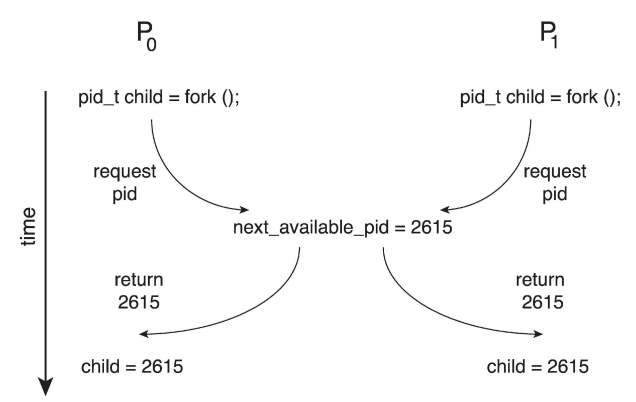
\includegraphics[width=.5\textwidth]{../res/imgs/synchronization/sim_fork_issue.png}
    \caption{Creazione di due processi figli con lo stesso \texttt{PID}.}
    \label{fig:sim_fork_issue}
\end{figure}
Supponiamo di avere una variabile, chiamata \texttt{next\_available\_pid} che contiene il primo \texttt{PID} disponibile. Se i due processi, in questo caso $P_0$ e $P_1$, fanno accesso alla variabile in maniera simultanea, verranno creati due figli con lo stesso \texttt{PID}. I due processi hanno fatto un accesso in maniera non esclusiva alla stessa zona di memoria condivisa generando quindi un problema.

Quello che abbiamo appena visto non è altro che un esempio di \textbf{critical section problem}. Generalizzando, possiamo dire che ogni processo è composto di un segmento di codice che deve avere un \textbf{accesso esclusivo} in quanto ha un accesso in scrittura dove aggiorna tabelle, modifica variabili o scrive su files. Di conseguenza si cerca di non interrompere un processo nel momento in cui questo è nella sua \textbf{sezione critica}.
% 
\subsubsection{Requisiti}\label{CS requisiti}
È stato stilato un elenco di 3 punti di requisiti che devono essere rispettati affinché non vengano generate situazioni dove un processo viene interrotto durante la sua sezione critica.
\begin{enumerate}
    \item \textbf{Mutua esclusione}: se il processo $P$ sta eseguendo la sua parte critica nessun altro processo deve interromperlo;
    \item \textbf{Progresso}: bisogna garantire che nessun processo rimanga in un'attesa perenne mentre aspetta la conclusione della parte critica di un altro processo. In altre parole, l'esecuzione della sezione critica di un processo non può essere posticipata in maniere indeterminata;
    \item \textbf{Attesa limitata}: deve esistere un limite massimo per cui un processo deve concludere la sua parte critica. 
\end{enumerate}
% 
\subsubsection{Soluzioni inefficienti}
Una prima idea banale è quella di \textbf{disabilitare} gli \textbf{interrupt} nel momento in cui un processo (un \textit{thread}) sta eseguendo la sua parte critica. Questa però è una soluzione poco elegante e anche poco funzionale. Si rischia infatti di far aspettare molto altri processi i quali necessitano di eseguire la loro sezione critica (starvation). 

Si è quindi pensato ad una soluzione un po' più elegante, ma che comunque è una forma embrionale rispetto a ciò che vedremo. Stiamo parlando di una semplice \textbf{soluzione software} tra due processi dove entrambi condividono una variabile \textit{booleana} \texttt{turn} che indica di chi è il turno per eseguire la sezione critica.
\begin{lstlisting}
while(true){
    while(turn == j); /* attendo che sia il mio turno */
    /* SEZIONE CRITICA */
    turn = j; /* rimando il turno all'altro processo */
    /* sezione rimasta */
}
\end{lstlisting}
Con questa soluzione, è rispettata la richiesta di mutua esclusione ma i punti (2) e (3) non sono rispettati: il processo \texttt{j} potrebbe anche durare un'ora e ci sarebbe un'ora di attesa. Non sono quindi i rispettati i limiti di attesa e nemmeno il progresso dei processi.
% 
\subsection{Soluzione di Peterson}
Una prima soluzione un po' più raffinata è quella di Peterson. In questa soluzione i due processi condividono due variabili:
\vspace{-5px}
\begin{itemize}
\setlength{\itemsep}{-.15 em}
    \item \texttt{turn} che è la variabile che indica di quale processo è il turno;
    \item \texttt{flag[2]} che è un array di due valori booleani che indicano se il processo i-esimo è pronto o meno per entrare nella sezione critica.
\end{itemize}

Come possiamo notare dal seguente segmento di codice, sono stati aggiunti alcuni controlli.
\begin{lstlisting}[caption={Soluzione di Peterson}]
while (true){
    flag[i] = true;
    turn = j;
    while (flag[j] && turn == j); /* aspetto fino a che non sono pronto e fino a che j non ha finito */
    /* SEZIONE CRITICA */
        flag[i] = false;
    /* sezione rimasta */
}
\end{lstlisting}
Osserviamo che possiamo intendere l'esecuzione della parte critica di un processo come una galleria a senso unico alternato: se un processo deve entrarci ma al suo interno ce n'è già un altro attende, altrimenti ci entra. L'esecuzione in "parallelo" è quindi mantenuta dato che un processo può essere molto lontano dalla galleria mentre il secondo la sta attraversando. Con questo modello, quindi, tutti e 3 i requisiti sono rispettati.
% 
\subsubsection{Architetture moderne}
Ciò nonostante, questa soluzione diventa obsoleta per i sistemi moderni \textit{multicore} e \textit{multithread}. Questo perché nelle architetture moderne il compilatore si prende la libertà di riordinare e riorganizzare il codice. Vediamo un esempio di due thread (assumiamo che le variabile condivise siano \texttt{x} e \texttt{flag}):
\begin{lstlisting}
/* THREAD 1 */
    while(!flag);
    print x

/* THREAD 2 */
    x = 100;
    flag = true;
\end{lstlisting}
Una volta eseguito il codice, ci aspettiamo che l'output sia \texttt{100}. Però, se le istruzioni nel thread 2 vengono invertite, il risultato è completamente diverso, perché il thread 1 viene eseguito prima che la variabile \texttt{x} venga cambiata a 100.
\begin{lstlisting}
/* THREAD 2 */
    flag = true;
    x = 100;
\end{lstlisting}

Al fine di fare in modo che la soluzione di Peterson funzioni anche nelle architetture moderne si introduce la \textbf{memory barrier}: questa è un'istruzione che rende le modifiche effettuate in memoria visibili a tutti i processori (\textit{cores}). Questo tipo di modello di memoria si dice \textit{strongly ordered}, ovvero una modifica in memoria è propagata immediatamente a tutti i core; si contrappone al \textit{weakly ordered} dove una modifica in memoria non è propagata istantaneamente. 

Con l'introduzione delle memory barrier ora la soluzione di Peterson rimane valida. Questo perché quando viene invocato un \texttt{memory\_barrier()} il sistema si assicura che tutti i load e store in memoria vengano completati prima di ogni altro load e store. Quindi anche se il codice venisse riordinato, la memory barrier si assicura che le modifiche in memoria siano completate. 
% 
\subsection{Sincronizzazione via hardware}
Tra le diverse soluzioni che abbiamo visto, la più gettonata rimane comunque l'implementazione di particolari \textbf{istruzioni hardware} che permettono di modificare il contenuto di una \textit{word} in memoria oppure di effettuare uno \textit{swap} di due word.

\subsubsection{Test and set}
La prima delle due istruzioni HW che discuteremo è la \texttt{test\_and\_set} dove prende un input booleano e lo memorizza in una variabile temporanea \texttt{tmp}; in secondo luogo il valore in ingresso viene settato a \texttt{true} e infine la variabile temporanea viene restituita. Lo pseoudcodice di quest istruzione è il seguente (ricordiamo che sono istruzioni a livello HW, quindi il codice è solo a scopo concettuale):
\begin{lstlisting}
boolean test_and_set(boolean *target){
    boolean tmp = *target;  /* salvo il valore di target */ 
    *target = true; /* setto a TRUE */
    return tmp;
}
\end{lstlisting}
Si osserva che dopo l'esecuzione dell'istruzione, il valore di \texttt{target} è sempre \texttt{true} e viene ritornato il vecchio valore della variabile in ingresso. Ricordiamo infine che è un'istruzione \textbf{atomica}, ciò significa che non può essere interrotta.

Vediamo ora come questa istruzione posso esserci utile per l'esecuzione della sezione critica di un processo:
\begin{lstlisting}[caption={Utilizzo \texttt{test\_and\_set}}]
while(true){
    while(test_and_set(&lock)); /* lock = true, attendo per la risolrsa, ora e' occupato.*/
        /* lock = false, posso cominciare a eseguire la parte critica perche' si e' liberato; metto lock = true*/
    /* SEZIONE CRITICA */
    lock = false; /* lock e' libero */ 
    /* sezione rimanente */
}
\end{lstlisting}
% 
\subsubsection{Compare and swap}
La seconda istruzione HW che andiamo a discutere si chiama \texttt{compare\_and\_swap} e, come per la precedente, anch'essa è un'istruzione atomica. Come vedremo, questa istruzione, ha ben 3 variabili in ingresso:
\vspace{-5px}
\begin{itemize}
\setlength{\itemsep}{-.15 em}
    \item \texttt{value}, che indica il valore da modificare;
    \item \texttt{expected}, che indica il valore che ci si aspetta contenga \texttt{value};
    \item \texttt{new\_value}, ovvero il nuovo valore con cui vogliamo cambiare \texttt{value}.
\end{itemize}
Osserviamo ora lo pseudocodice dell'istruzione:
\begin{lstlisting}
int compare_and_swap(int *value, int expected, int new_value){
    int tmp = *value;
    if (*value == expected)
        *value = new_value;
    return temp; /* ritorna vecchio valore di value */
}
\end{lstlisting}
Notiamo che, a differenza di \texttt{test\_and\_set}, in questo caso il valore di \texttt{value} viene modificato solo nel momento in cui coincide con il valore che ci aspettiamo questo viene modificato con il valore inserito (\texttt{new\_value}). Capiamo ora come questa istruzione possa essere utilizzata per la gestione della sezione critica e come questa sia più \textbf{flessibile} rispetto alla precedente.
\begin{lstlisting}[caption={Utilizzo di \texttt{compare\_and\_swap}}]
while(true){
    while(compare_and_swap(&lock, 0, 1) != 0); 
        /* lock = 1 = true, continuo ad aspettare */
        /* lock = 0 = false, viene ritornato 0, quindi esco dal while, e occupo lo spazio, lock = 1 */
    /* SEZIONE CRITICA */
    lock = 0;
    /* sezione rimasta*/
}
\end{lstlisting}

% 
\subsubsection{Variabili atomiche}
Istruzioni come \texttt{compare\_and\_swap} sono utilizzate per comporre dei blocchi per comporre altri oggetti di sincronizzazione. Uno tra questi oggetti è la variabile atomica che fornisce degli aggiornamenti elementare a dei dati primitivi. Segue infatti l'esempio di \texttt{increment()} dove il valore intero \texttt{v} viene incrementato senza interruzioni
\begin{lstlisting}[caption={Esempio di una variabile atomica \texttt{increment()}}]
void increment(atomic_int *v){
    int temp;
    do{
        temp = *v;
    } while (temp != compare_and_swap(v, temp, temp+1));
}
\end{lstlisting}
% 
\subsection{Mutex lock e Semafori}
Le soluzioni che abbiamo visto in precedenza erano intricate e spesso non erano accessibili da applicazioni esterni; inoltre creano ulteriori complicazioni in sistemi multithreading. A questo proposito i progettisti di sistemi operativi hanno costruito diversi \textit{tool} al fine di risolvere il problema della sezione critica.

Il primo che andremo a vedere è il \textbf{mutex lock} (\textbf{MUT}ual \textbf{EX}clusion lock) che è una variabile booleana che indica se il \textbf{lock}, ovvero la sezione critica è disponibile o meno. Questa è protetta da due istruzioni atomiche di acquisizione e rilascio:
\vspace{-5px}
\begin{itemize}
\setlength{\itemsep}{-.15 em}
    \item \texttt{acquire()} che blocca la \textit{CS}\footnote{\textit{CS} sta per \textit{Critic Session}, ovvero sezione critica};
    \item \texttt{release()} che rilascia il lucchetto e quindi la \textit{CS} è liberata.
\end{itemize}
Spesso queste sono implementate via HW attraverso istruzioni come \texttt{compare\_and\_ swap}.

Come possiamo notare dallo pseudocidce sottostante, ci troviamo in una situazione di \textbf{busy waiting} in quanto il thread continua ad entrare nel ciclo fino a che non acquisisce il lucchetto. È evidente che stiamo sprecando CPU, che potrebbe essere usata per altri thread.
\begin{lstlisting}
while(true){
    acquire();
    /* SEZIONE CRITICA */
    release();
    /* sezione rimanente */
}
\end{lstlisting}

A questo proposito, questa pratica è raffinata tramite i \textbf{semafori}, che non sono altro che una \textbf{variabile intera} (\texttt{S}) accessibile, anche in questo caso attraverso due operazioni atomiche: \texttt{wait()} e \texttt{signal()}.
\begin{lstlisting}
wait(S){
    while (S<=0); /* busy wait */
    S--;
}

signal(S){
    S++;
}
\end{lstlisting}
Se la variabile \texttt{S} può assumere solo il valore di 0 o 1, si parla di semafori \textbf{binari} (ovvero dei mutex lock), altrimenti si fa riferimento ai \textbf{counting semaphores}. 

Attraverso i semafori abbiamo la possibilità di fare eseguire una parte di processo prima che un altro processo inizi. Siano $P_1$ e $P_2$ due processi che contengono il segmento $S_1$ ed $S_2$; per fare in modo che $S_1$ sia eseguito prima di $S_2$ possiamo utilizzare i semafori.
\begin{lstlisting}
P1:
    S1;     /* eseguo S1 */
    signal(synch); /* dico a P2 che ho finito */

P2:
    /* busy wait */
    wait(synch); /* aspetto che P1 abbia finito */
    S2;     /* eseguo S2 */
\end{lstlisting}
Possiamo notare però che anche in questo caso $P_2$ è in una fase di busy waiting.

\subsubsection{Waiting queue}
Per evitare che accada è necessario implementare una \textbf{waiting queue}:
\begin{lstlisting}[caption={Struttura del semaforo con waiting queue}]
typedef struct {
    int value;
    struct process *list;   /* indica la prossima entry nella lista */
} semaphore
\end{lstlisting}
Qui abbiamo a disposizione altre due operazioni per implementare la sincronizzazione tra processi:
\vspace{-5px}
\begin{itemize}
\setlength{\itemsep}{-.15 em}
    \item \texttt{sleep()} che mette a dormire il processo o il thread e lo inserisce nella waiting queue;
    \item \texttt{wakeup()} che rimuove il primo processo della coda e lo inserisce nella \textit{ready queue}, coda che contiene i processi pronti per essere eseguiti.
\end{itemize}

A questo punto possiamo ridefinire le due operazioni basi del semaforo: \texttt{wait} e \texttt{signal}.
\begin{lstlisting}[caption={Utilizzo di semaforo con \textit{waiting queue}}]
wait(semaphore *s){
    S->value--;     /* decremento il valore del semaforo */
    if (S->value < 0){
        aggiungi processo in S->list;
        sleep();    /* evito il busy waiting, mi tolgo dalla CPU e aspetto che signal() mi svegli dalla coda */
    }
}

signal(semaphore *S){
    S->value++;     /* incremento il valore del semaforo */
    if (S->value <= 0){
        rimuovii processo in S->list;
        wakeup();
    }
}
\end{lstlisting}

Bisogna però fare attenzione a utilizzare \texttt{wait} e \texttt{signal} nel modo corretto: non si può prima invocare \texttt{signal} e poi \texttt{wait} oppure invocare \texttt{wait} due volte di seguito. Questo utilizzo incorretto delle due operazioni può generare errori.
% 
\subsection{Monitor}
Cerchiamo ora di risolvere il problema dei semafori: le operazioni di \texttt{wait} e \texttt{signal} erano lasciate al programmatore. Questa scelta ha come unica conseguenza la generazione di errori da parte dell'utilizzatore (che, come vedremo più avanti prendono il nome di \textbf{deadlock}, capitolo \ref{deadlocks}). Cerchiamo quindi di implementare un'astrazione dei semafori al fine di limitarne i danni. Queste astrazioni di alto livello sono proprio i \textbf{monitor} i quali garantiscono l'esecuzione di un processo alla volta.

\subsubsection{Struttura e implementazione}
La struttura di astrazione del monitor è formata da una variabile condivisa da tutti i processi, da del codice di inizializzazione per il monitor e da tante funzioni o procedure (ogni processo ha le stesse procedure).
\begin{lstlisting}[caption={Struttura del monitor}]
monitor name{
    /* dichiarazione della variabile condivisa */
    codice di inizializzazione (...) { ... }

    procedura F1 (...) { ... }
    procedura F2 (...) { ... }
    /* ... */ 
    procedura Fn (...) { ... }    
}
\end{lstlisting}
Come possiamo osservare dalla figura \ref{fig:monitor}, concettualmente, il monitor raggruppa tutti i processi attraverso dei dati condivisi in una coda.
\begin{figure}[!h]
    \centering
    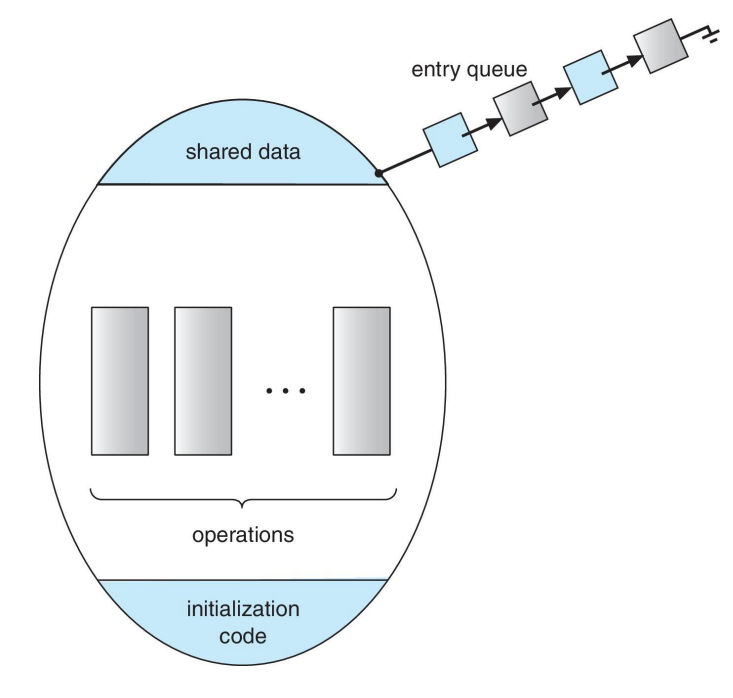
\includegraphics[width=.55\textwidth]{../res/imgs/synchronization/monitor.png}
    \caption{La struttura di astrazione del monitor.}
    \label{fig:monitor}
\end{figure}

Per implementare un monitor ci appoggiamo sui semafori, in particolare su un mutex:
\begin{lstlisting}
semaphore mutex = 1;    /* semaforo binario = mutex */

wait(mutex) /* aspetto che il mutex si liberi per occuparlo */
    /* corpo della funzione Fi */
signal(mutex) /* libero il mutex **/
\end{lstlisting}
È quindi necessario modificare ogni procedura del monitor bloccando e poi rilasciando il mutex. In questo modo, a differenza dei semafori, le operazioni di \texttt{wait} e \texttt{signal} sono già implementate all'interno delle procedure che eseguono quelle operazioni, al posto del programmatore. Un esempio di utilizzo completo è presente nella sezione \ref{utilizzo monitor}.

\subsubsection{Variabile di condizione}
Oltre alla struttura base, illustrata nel paragrafo precedente, possiamo anche inserire le \textit{condition variables}  (rappresentazione in figura \ref{fig:condition_variable}) che possono eseguire le stesse due operazioni dei semafori: \texttt{wait} e \texttt{signal}.
\begin{figure}[!h]
    \centering
    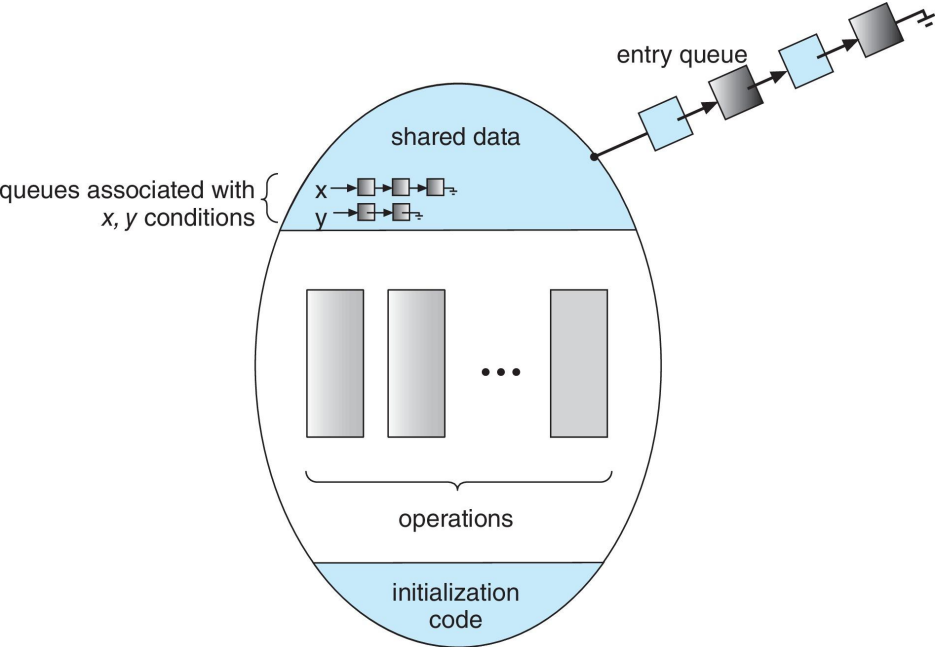
\includegraphics[width = .65\textwidth]{../res/imgs/synchronization/condition_variable.png}
    \caption{Caption}
    \label{fig:condition_variable}
\end{figure}
In questo caso però le due operazioni sono modificate e non portano ad errori se utilizzate male. Ricordiamo che, nel caso dei semafori, se \texttt{signal} fosse stato invocato senza aver prima invocato il corrispettivo \texttt{wait}, avrebbe erroneamente incrementato il contatore. In questo caso invece, se non è presente alcun processo in \texttt{wait}, allora \texttt{signal} non fa nulla.

Emerge ora un piccolo dubbio. Se ci sono diversi processi che sono in \texttt{wait}, quando viene effettuato un \texttt{x.signal()}, quale di questi processi viene eseguito per prima? Notiamo che ci troviamo in una situazione molto simile allo scheduling (capitolo \ref{CPU scheduling}) solo che, in questo caso non è più a livello di sistema operativo ma è a livello di monitor e di accesso alla sezione critica. Per risolvere questo problema ci possono essere algoritmi come FCFS oppure a livello di priorità: chi ha la priorità più alta viene fatto eseguire prima. Spesso la priorità è definita in base al tempo di utilizzo della sezione critica, ma si fa presente che se entrano nella coda processi con un tempo di utilizzo molto breve, i processi con un utilizzo lungo possono essere in attesa perenne ed andare in \textbf{stravation}. Ecco che non viene più rispettato il terzo requisito, ovvero che l'attesa di un processo per la sezione critica deve essere limitata (vedi paragrafo \ref{CS requisiti}).
% 
\subsection{Problemi comuni della sincronizzazione}


\subsubsection{Buffer limitato}
Il primo problema che andiamo a discutere è il problema del buffer limitato. Abbiamo a disposizione un buffer che contiene \textit{n} elementi, ovvero il numero di processi in coda per accedere alla loro sezione critica. Disponiamo inoltre di tre semafori:
\vspace{-5px}
\begin{itemize}
\setlength{\itemsep}{-.15 em}
    \item \texttt{mutex} che consente l'accesso al buffer in maniera esclusiva (inizializzato ad 1);
    \item \texttt{full} che segnala in numero di elementi contenuti all'interno del buffer (inizializzato a 0);
    \item \texttt{empty} che indica la quantità di spazi disponibili all'interno del buffer, sarebbe \textit{n - }\texttt{full} (inizializzato ad \textit{n}).
\end{itemize}
Analizziamo la soluzione del problema, che è molto simile al problema del produttore e consumatore.
\begin{lstlisting}[caption = {Problema del buffer limitato}]
/* Produttore */
while (true){
    /* produco un elemento */
    wait(empty); /* aspetto che ci sia spazio all'interno del buffer, ovvero che ci sia almeno una locazione libera (empty > 0) */
    wait(mutex); /* ora che c'e' un posto libero, richiedo l'accesso alla sezione critica */
    /* SEZIONE CRITICA: aggiungo il codice nel buffer */
    signal(mutex); /* libero la sezione critica */
    signal(full); /* incremento di 1 il numero di elementi nel buffer
}

/* Consumatore */
while(true){
    wait(full); /* aspetto che ci siano >0 elementi nel buffer */
    wait(mutex); /* aspetto l'accesso esclusivo nel buffer */
    /* SEZIONE CRITICA: rimuovo l'elemento dal buffer */
    signal(mutex); /* libero la sezione critica */
    signal(empty); /* incremento il numero di locazioni libere */
}
\end{lstlisting}

Osserviamo che i comando \texttt{wait(empty)} e \texttt{wait(mutex)} all'interno di produttore \textbf{non} possono essere invertiti. Se prima infatti viene bloccato il mutex, il consumatore non sarà più in grado di liberare il buffer che, se è pieno, porta ad un'attesa perenne il produttore in \texttt{wait(empty)}: siamo ricaduti in una situazione di \textit{deadlock}.

% 
\subsubsection{Problema dei lettori e degli scrittori}
Il secondo problema è detto dei lettori e degli scrittori. In questo caso: (1) più lettori possono leggere lo stesso dataset (che può essere anche un file su disco) contemporaneamente (per definizione, non possono modificarlo) e (2) lo scritture deve poter scrivere sul dataset senza che quest'ultimo venga letto. Solo nel momento in cui ha terminato (mutua esclusione), allora i lettori possono effettuare nuovamente l'accesso simultaneo. 

Non ci soffermiamo sul codice, ci limitiamo a dire che è sufficiente utilizzare due semafori:
\vspace{-5px}
\begin{itemize}
\setlength{\itemsep}{-.25 em}
    \item \texttt{rw\_mutex}, semaforo binario inizializzato ad 1, che indica che la risorsa è occupata dallo scrittore;
    \item \texttt{mutex}, anch'esso un semaforo binario che segnala che la risorsa è in lettura da almeno un lettore;
    \item \texttt{read\_count}, un intero che conta il numero di lettore che stanno leggendo la risorsa.
\end{itemize}

In questo caso i problemi generati sono due. Il primo è che c'è la possibilità che lo scrittore non riesce mai ad effettuare l'accesso, entra quindi in una fase di attesa perenne. Il secondo problema che emerge è che quando lo scrittore ha effettuato l'accesso, nessun lettore è in grado di accedere: anche in questo caso si può ricadere in una fase di \textit{starvation}.

% 
\subsubsection{Problema dei 5 filosofi}\label{5_filosofi}
Il problema dei 5 filosofi, rimane il più conosciuto (e il più importante).
\begin{figure}[t!]
    \centering
    
\includegraphics[width = .5\textwidth]{../res/imgs/synchronization/5_filosofi.png}
    \caption{Disposizione dei 5 filosofi.}
    \label{fig:5_filosofi}
\end{figure}
Un filosofo, può pensare o mangiare. Facendo riferimento alla figura \ref{fig:5_filosofi}, osserviamo che i filosofi sono disposti in un tavolo rotondo che ha al centro una scodella di riso (che allegoricamente indica il dataset, ovvero la risorsa condivisa). Alla destra e alla sinistra di ciascun filosofo è presente una bacchetta: questa rappresenta il semaforo in quanto se un filosofo smette di pensare e inizia a mangiare, non può farlo se il filosofo alla sua sinistra o alla sua destra sta mangiando, in quanto almeno una delle due bacchette sono occupate.

Proviamo a dare una prima soluzione a questo problema di sincronizzazione con i semafori. 
\begin{lstlisting}[caption = {Risoluzione del problema dei  filosofi con i semafori}]
while(true){
    wait(chopstick[i]); /* attende la bacchetta a sinistra */
    wait(chopstick[ (i + 1) % 5]); /* attende la bacchetta a destra */
    /* SEZIONE CRITICA: mangia dalla ciotola di riso */
    signal(chopstick[i]); /* rilascia la bacchetta a sx */
    signal(chopstick[ (i + 1) % 5]); /* rilascia la bacchetta a dx */
    /* pensa */
}
\end{lstlisting}
Sembrerebbe tutto ottimo, ma cosa succede se tutti e 5 i filosofi prendono la loro bacchetto sinistra allo stesso tempo? Entrano in una situazione di attesa infinita (deadlock) un quanto tutte le loro bacchette destre sono occupate dal filosofo alla loro destra. Proviamo a risolvere questo nuovo problema attraverso i \textbf{monitor}.\label{utilizzo monitor}
\begin{lstlisting}[caption = {Risoluzione del problema dei  filosofi con i monitor}]
monitor DiningPhilosophers{  /* creo la struttura astratta */
    enum { THINKING, HUNGRY, EATING } state[5]; /* per ogni filosofo e' definito lo stato in cui si trova */
    condition self[5];  /* condition variable */

    void test(int i){
        if ((state[(i + 4) % 5] != EATING) /* se il vicino di sinistra non sta mangiano */ &&
            (state[i] == HUNGRY) /* se ho fame */ &&
            (state[(i + 1) % 5] != EATING)) /* se il vicino di destra non sta mangiando */ {
                state[i] = EATING; /* mi metto a mangiare */
                self[i].signal();
            }
    }

    void pickup(int i){ /* acquire */
        state[i]  = HUNGRY;
        test(i); /* se posso, mi metto a mangiare */
        if (state[i] != EATING) /* se non sto mangiando */
            self[i].wait(); /* mi metto in attesa*/
    }

    void putdown(int i){ /* release */
        state[i] = THINKING; /* mi rimetto a pensare */
        /* controllo che il mio vicino sinistro e destro non siano in attesa */
        test((i + 4) % 5);
        test((i + 1) % 5);
    }

    initialization_code(){ /* all'inizio tutti i filosofi stanno pensando */
        for (int i = 0; i < 5; i++)
            state[i] = THINKING; 
    }
}

\end{lstlisting}
Dopo aver implementato questa struttura astratta è semplicemente necessario utilizzare le due operazione \texttt{pickup()} e \texttt{putdown()} al fine di fare in modo che tutti i filosofi mangino sincronizzati. Ad ogni modo, anche in una situazione così raffinata la \textbf{starvation} è possibile, nel caso in cui un filosofo si metta a mangiare e non smetta più.
\begin{lstlisting}
DiningPhilosophers.pickup(i);
    /* SEZIONE CRITICA (mangio) */
DiningPhilosophers.putdown(i);
\end{lstlisting}
